\documentclass[resume]{subfiles}



% 1) Protocoles en couches
% 2) Modèle OSI
% 3) Couches OSI
% 4) Fonctionnement du modèle OSI
% 5) IEEE802.15.4
% 6) Stratégies d'implémentation

\begin{document}
\section{Introduction}
\subsection{OSI}

\begin{figure}[H]
\centering
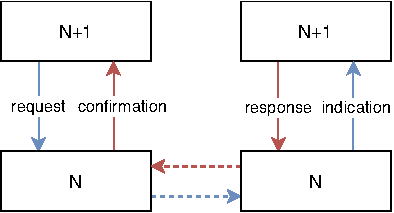
\includegraphics[width=5cm,page=1]{Schemas-crop.pdf}
\end{figure}
\begin{figure}[H]
\centering
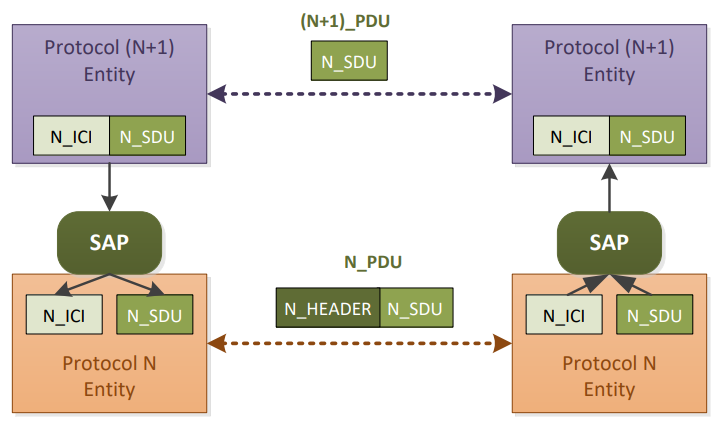
\includegraphics[width=5cm,page=1]{img_1.png}
\end{figure}
Un SAPI permet de choisir quel protocole utiliser (si il y a plusieurs protocoles)



\end{document}